\documentclass[11pt]{preprint}

\setlength{\topmargin}{0mm} \setlength{\oddsidemargin}{0mm}
\setlength{\textwidth}{160mm} \setlength{\textheight}{215mm}

\usepackage{amssymb,amsmath,amscd,amsthm}
\usepackage{tikz}

\newtheorem{proposition}{Proposition}

\def\enumb{\begin{enumerate}}
\def\enume{\end{enumerate}}
\def\integers{\mathbb{Z}}
\def\multiset#1#2{\ensuremath{\left(\kern-.3em\left(\genfrac{}{}{0pt}{}{#1}{#2}\right)\kern-.3em\right)}}

\title{Discrete Mathematics, 2016 Spring - HW 6}
\author{Instructor: Zsolt Pajor-Gyulai}
\institute{Courant Institute of Mathematical Sciences, NYU}



\begin{document}

\maketitle

To get full credit  in all of the problems, use rigorous justification and unless otherwise indicated, make sure that your solution reads as a perfect English sentence. You should only assume integers, operations and order relations as given. If you use a statement or a definition from the textbook, make sure to indicate it.
\vspace{0.2cm}

\textbf{Section 20}
\enumb
\item[1)] Please state the contrapositive of each of the following statements:
\enumb
\item If $p$ is prime, the $2^p-2$ is divisible by $p$.
\item If the diagonals of a parallelogram are perpendicular, then the parallelogram is a rhombus.
\item If the battery is fully charged, the car will start.
\item If $A$ or $B$, then $C$.
\enume
\item[10)] Prove by contradiction: Let $a$ be a number with $a>1$. Prove that $\sqrt{a}$ is strictly between $1$ and $a$.
%\item[12)] Prove by contradiction: A positive integer is divisible by $10$ if and only if its last digit (when written in base ten) is a zero. You  may assume that every positive integer $N$ can be expressed as:
%\[
%N=d_k10^k+d_{k-1}10^{k-1}+\dots+d_1 10+d_0
%\]
%where the numbers $d_0$ through $d_k$ are in the set $\{0,1,\dots,9\}$ and $d_k\neq 0$. In this notation, $d_0$ is the one's digit of $N$'s base ten representation.
%\item[15)] Prove the converse of the Addition Principle. The converse of a statement ``If $A$, then $B$'' is the statement ``If $B$, then $A$.'' In other words, your job is to prove the following: Let $A$ and $B$ be finite sets. If $|A\cup B|=|A|+|B|$, then $A\cap B=\emptyset$.
\enume
\textbf{Section 21}
\enumb
\item[4-5)] Prove the following statements by smallest counterexample 
\enumb
\item $n!\leq n^n$ for all positive integers $n$.
\item $\binom{2n}{n}\leq 4^n$ for all natural numbers $n$.
\enume

\item[7)] The \textbf{Fibonacci numbers} are the list of integers $(1,1,2,3,5,8,\dots)=(F_0,F_1,F_2,\dots)$ where 
\[
F_0=1,\qquad F_1=1,\qquad F_n=F_{n-1}+F_{n-2}, \textrm{ for $n\geq 2$}.
\]
\enumb
\item Read the proof of the fact that for all $n\in\mathbb{N}$, we have $F_n\leq 1.7^n$ on p133 in the textbook.
\item Now prove using the smallest counterexample method that $F_n>1.6^n$ whenever $n\geq 29$.
\enume
\enume
\newpage
\textbf{Section 22}
\enumb
\item[4-5,16)] Prove the following equations and inequalities by induction.
\enumb
\item $1^3+2^3+\dots n^3=\frac{n^2(n+1)^2}{4}$.
\item $1+\frac{1}{2}+\frac{1}{3}+\dots+\frac{1}{2^n}\geq 1+\frac{n}{2}$
\enume
\item[10)] Prove, by induction, that the sum of the angles of a convex $n$-gon (with $n\geq 3$) is $180(n-2)$ degrees.

\item[12)] The \textit{Towers of Hanoi} is a puzzle consisting of a board with three dowels and a collection of $n$ disks of $n$ different sizes (radii). The disks have holes drilled through their centers so that they can fit on the dowels on the board. Initially, all the disks are on the first dowel and are arranged in size order (from the largest on the bottom to the smallest on the top).

\begin{figure}[h]
\centering
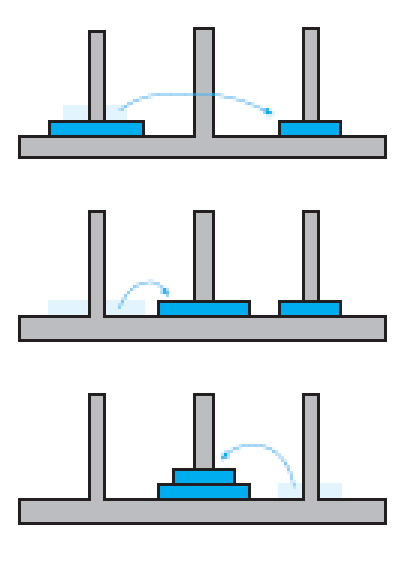
\includegraphics{Hanoi.jpg}
\caption{Solution of the Towers of Hanoi puzzle for $n=2$.}
\end{figure}

The object is to move all the disks to another dowel in as few moves as possible. Each moves consists of taking the top disk off one of the stacks and placing it on another stack, with the added condition that you may not place a larger disk atop a smaller one. The figure shows how to solve the puzzle in three moves when $n=2$. Prove that for every positive integer $n$, the puzzle can be solved in $2^n-1$ moves.
\enume
\end{document}